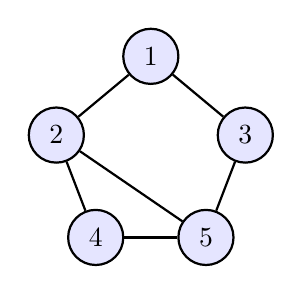
\begin{tikzpicture}[
  vnode/.style={circle, draw, minimum size=7mm, inner sep=0pt, fill=blue!10},
  thick
]
  \node[vnode] (1) at (0, 1.5) {1};
  \node[vnode] (2) at (-1.2, 0.5) {2};
  \node[vnode] (3) at (1.2, 0.5) {3};
  \node[vnode] (4) at (-0.7, -0.8) {4};
  \node[vnode] (5) at (0.7, -0.8) {5};
  
  \draw (1) -- (2);
  \draw (1) -- (3);
  \draw (2) -- (4);
  \draw (3) -- (5);
  \draw (4) -- (5);
  \draw (2) -- (5);
\end{tikzpicture}
\par\medskip
\textit{Obrázek 1.1: Příklad neorientovaného grafu s 5 vrcholy a 6 hranami.}
